\documentclass[11pt]{beamer}

%%%%%%%% tema e cor %%%%%%%%
\mode<presentation> {
\usetheme{Madrid}
\usecolortheme{rose}
}

\usepackage[english]{babel}
\usepackage[utf8]{inputenc}
\usepackage{graphicx} 
\usepackage{booktabs} 

%
%{
%================= logos no meio =====================
%\vspace*{-0.35cm}
%\includegraphics[width=1.8cm]{img/logo-uea.png}
%\hspace*{0.25cm}~%
%\includegraphics[width=1.8cm]{img/logo-neo.png}
%\vspace*{0.35cm}\\
%Núcleo de Engenharia e Otimização -- NEO \\
%Escola Superior de Tecnologia -- EST\\
%Universidade do Estado do Amazonas -- UEA\\
%%\medskip
%%\texttt{\{lods.eng,ronety\}@uea.edu.br} % emails
%}
\date{\today}

\AtBeginSection[]
{
\begin{frame}
\frametitle{Table of contents}
\tableofcontents[currentsection]
\end{frame}
}

%%%%%%%% Packages %%%%%%%%%
\usepackage{float}
\usepackage{subfig} %Subplots
\usepackage{graphicx}
\usepackage{hyperref}

%%%%%%%% title and subtitle %%%%%%%%
\title[ProbCons]{ProbCons: Probabilistic consistency-based multiple sequence alignment} 

%%%%%%%% name %%%%%%%%
\author[Group 5]{Álvaro Huertas García \\ Diego Mañanes Cayero
                 \\ Alejandro Martín Muñoz \\ Sara Dorado Alfaro} 

\begin{document}

\frame{\titlepage}
\begin{frame}
    \frametitle{Table of contents}
    \tableofcontents
\end{frame}

%%%%%%%% slides %%%%%%%%
\section{Introduction} 
\begin{frame}{Introduction $\rightarrow$ 2 Frequency dependent fitness}

    \begin{itemize}    
        \item Game theory.
        \item $OncoSimulR$ model $\rightarrow$ the fitness of a subpopulation will depend on the relative abundance of the different subpopulations.
        \item The fitness of each subpopulation is defined as an arbitrary function of the genetic interactions between multiple genes.       
    \end{itemize}
    
\end{frame}

\begin{frame}{Introduction $\rightarrow$ Effects on fitness}

    \begin{itemize}
        \item $allFitnessEffects$ function:
        \begin{itemize}
            \item $genoFitness$ = dataframe
            \begin{itemize}
                \item First column: genotypes.
                \item Second column: expressions for the functions that relate fitness to frequencies of other genotypes.
            \end{itemize}
            \item $frequencyDependentFitness$ = TRUE
            \item $frequencyType$ = “rel” or $frequencyType$ = “abs”
            \item $spPopSizes$
        \end{itemize}        
    \end{itemize}

\end{frame}

\begin{frame}{Introduction $\rightarrow$ Assess fitness}

    \begin{itemize}
        \item $evalGenotype$ function:
        \begin{itemize}
            \item $fitnessEffects$ = $allFitnessEffects$ object
            \item $genotype$
        \end{itemize}
        \item $evalAllGenotypes$ function:
        \begin{itemize}
            \item $fitnessEffects$ = $allFitnessEffects$ object
        \end{itemize}
    \end{itemize}
    
\end{frame}

\begin{frame}{Introduction $\rightarrow$ Perform simulations}

    \begin{itemize}
        \item $oncoSimulIndiv$ and $oncoSimulPop$ functions.
    \end{itemize}
    \begin{columns}
        \begin{column}{0.5\textwidth}
            \begin{figure}[t]
                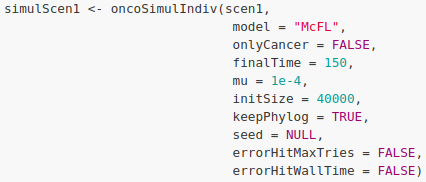
\includegraphics[width=0.9\linewidth]{img/oncoSimulIndiv.png}
            \end{figure}
        \end{column}
        \begin{column}{0.5\textwidth}
            \begin{figure}[t]
                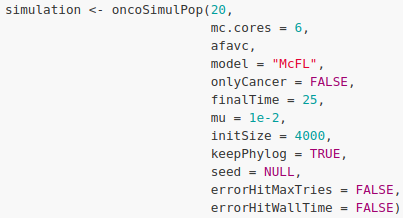
\includegraphics[width=0.9\linewidth]{img/oncoSimulPop.png}
            \end{figure}
        \end{column}
    \end{columns}
    
\end{frame}

\section{Types of aligners}
\subsection{Additional functions}

\begin{frame}{Additional functions: graphical summary}
    \begin{itemize}
        \item \textbf{Box-plot:} graphical summary of the distribution of simulations results
    \end{itemize}
    \textbf{}
    \begin{figure}[t]
        \centering
        \textbf{compositionPop2()}\par\medskip
        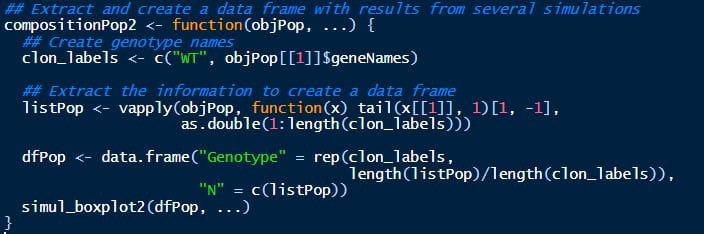
\includegraphics[width=0.9\linewidth]{img/compositionPop2.PNG}
        \caption{Code for compositionPop2() function}
    \end{figure}
\end{frame}

\begin{frame}{Additional functions: graphical summary}
    \begin{figure}[t]
        \centering
        \textbf{simul\_boxplot2()}\par\medskip
        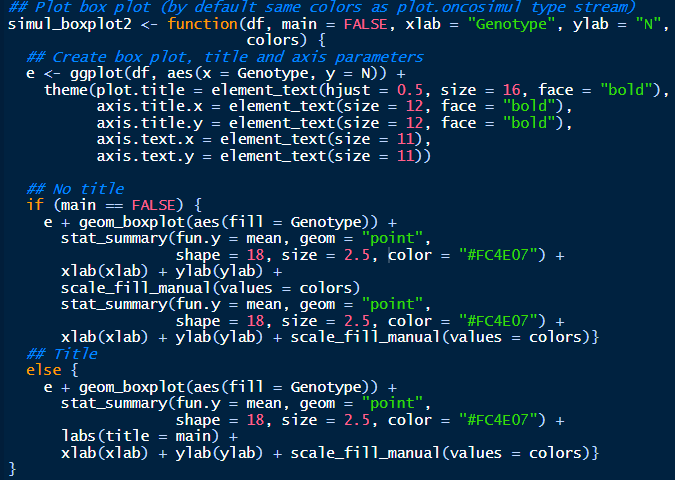
\includegraphics[width=0.65\linewidth]{img/simul_boxplot.PNG}
        \caption{Code for simul\_boxplot2() function}
    \end{figure}
\end{frame}

\begin{frame}{Additional functions: graphical summary}
    \begin{figure}
    \centering
    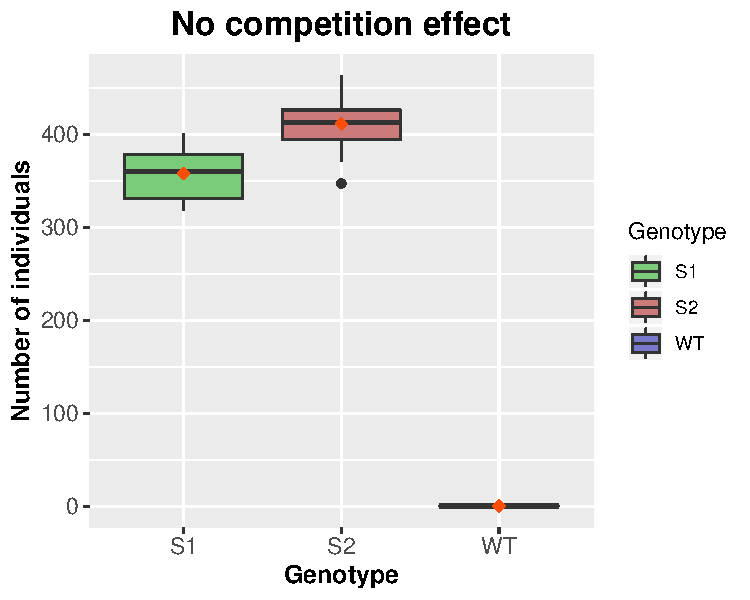
\includegraphics[width=0.65\linewidth]{img/boxplot_example.pdf}
    \caption{Box-plot from one of the Lotka-Volterra's example. 20 simulations were made}
    \end{figure}
\end{frame}

\begin{frame}{Additional functions: graphical summary}
    \begin{itemize}
    \item \textbf{Stripchart:} summary of simulations with oscillating trajectories
     \end{itemize}
     \begin{figure}
        \centering
        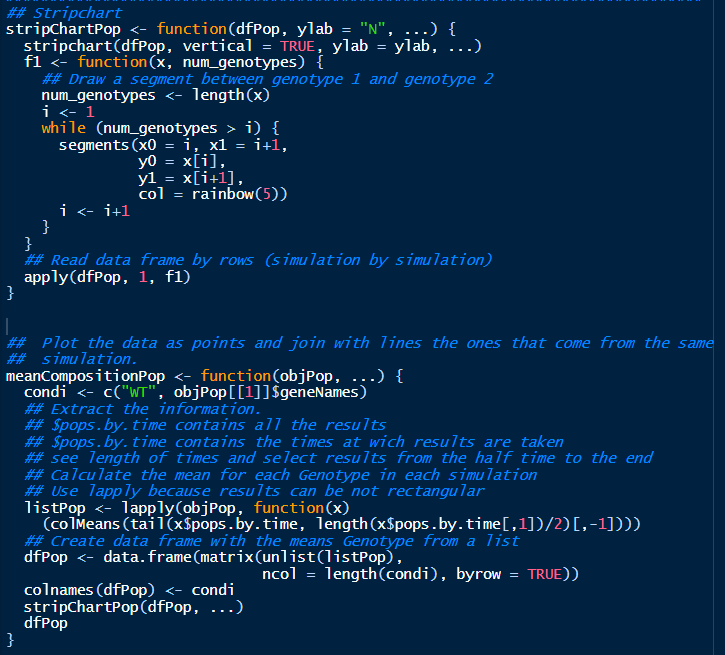
\includegraphics[width=0.6\linewidth]{img/stripchart_code.PNG}
        \caption{stripChartPop() and meanCompositionPop() code}
    \end{figure}
\end{frame}

\begin{frame}{Additional functions: graphical summary}
    \begin{figure}
    \centering
    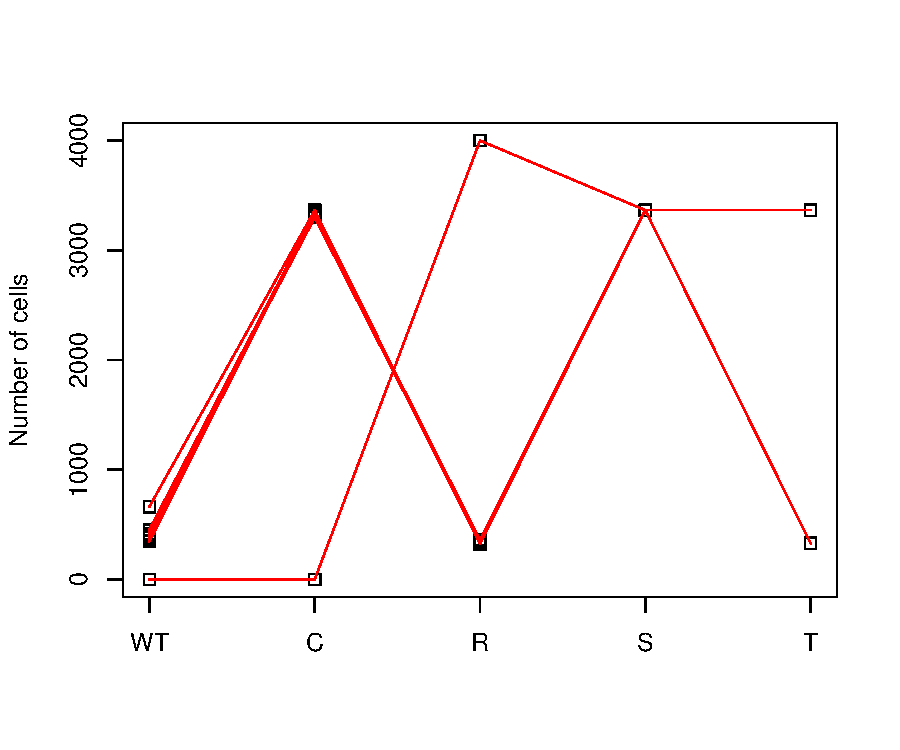
\includegraphics[width=0.8\linewidth]{img/stripchart_example.pdf}
    \caption{Example of the graphical summary of an oscillating trajectory}
    \end{figure}
\end{frame}

\subsection{Modification of the code}

\begin{frame}{Modification of the code}
	\begin{itemize}
		\item \textbf{Legend location}: plot.oncosimul and plotClonesSt
	\end{itemize}
    \begin{figure}
    \centering
    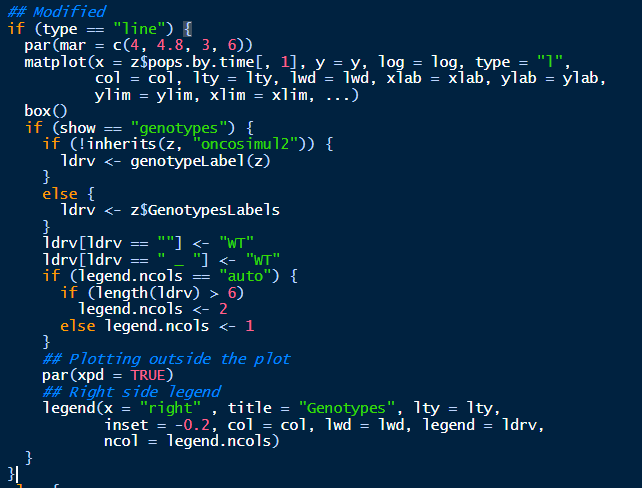
\includegraphics[width=0.7\linewidth]{img/plot_legend_outside.PNG}
    \caption{Par settings for placing the legend outside}
    \end{figure}
\end{frame}

\begin{frame}{Modification of the code}
	\begin{itemize}
		\item \textbf{Legend location}
	\end{itemize}
	\begin{columns}
		\begin{column}{0.5\textwidth}
			\begin{figure}
				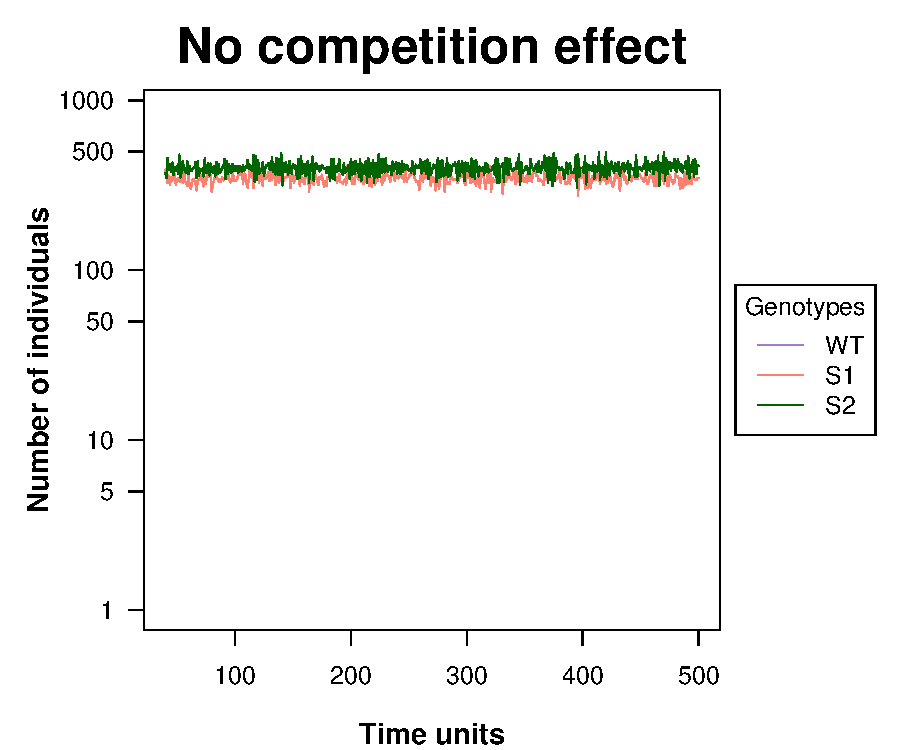
\includegraphics[width=0.95\linewidth]{img/line_example.pdf}
			\end{figure}
		\end{column}
		\begin{column}{0.5\textwidth}
			\begin{figure}
				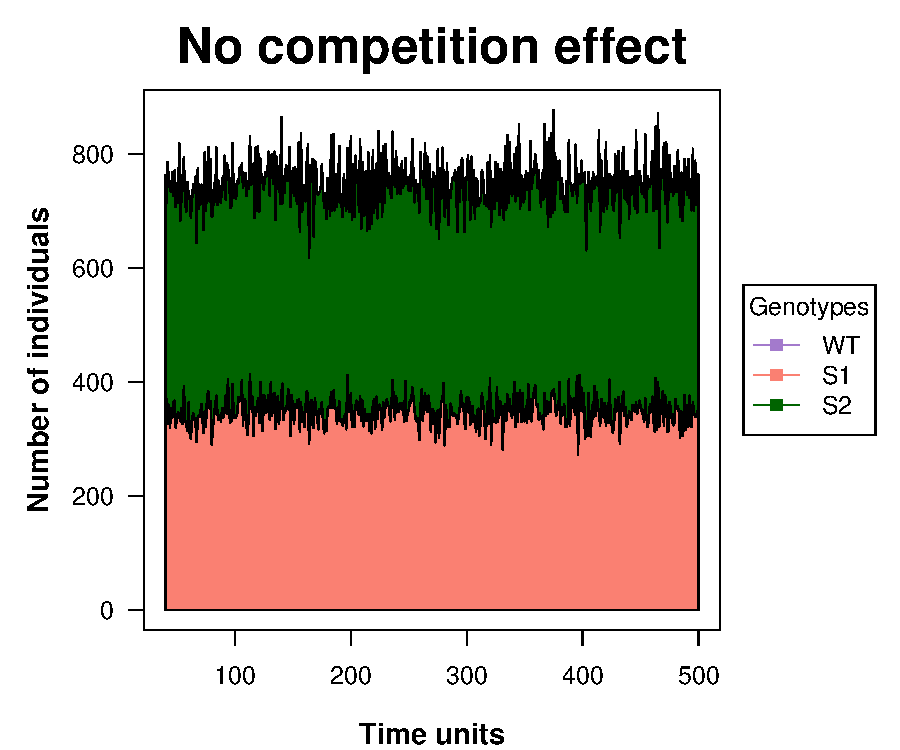
\includegraphics[width=0.95\linewidth]{img/stream_example.pdf}
			\end{figure}
		\end{column}
	\end{columns}
\end{frame}


\section{Consistency-based approaches}
\subsection{List of experiments}

\begin{frame}{List of experiments}
	\begin{enumerate}
		\item <alert@2> Rock-paper-scissors model in bacterial community
		\item Evolutionary games theory: Hawk and Dove example
		\item The Lotka-Volterra model of competition between two competing species
		\item Game Theory with social dilemmas of tumour acidity and vasculature
		\item Prostate cancer tumour–stroma interactions
		\item <alert@2> Evolutionary Dynamics of Tumor-Stroma Interactions in Multiple Myeloma
	\end{enumerate}
\end{frame}

\subsection{An experiment with bacteria}

\begin{frame}{Rock-paper-scissors game in bacterial community}

    \begin{itemize}
        \item \textbf{Title:} Local dispersal promotes biodiversity in a real-life game of rock–paper–scissors.
        \item \textbf{Authors:} Benjamin Kerr, Margaret A. Riley, Marcus W. Feldman, Brendan J. M. Bohannan.
        \item Three competing species of bacterias with relationships similar to rock-paper-scissors game.
    \end{itemize}
            \begin{figure}[t]
    			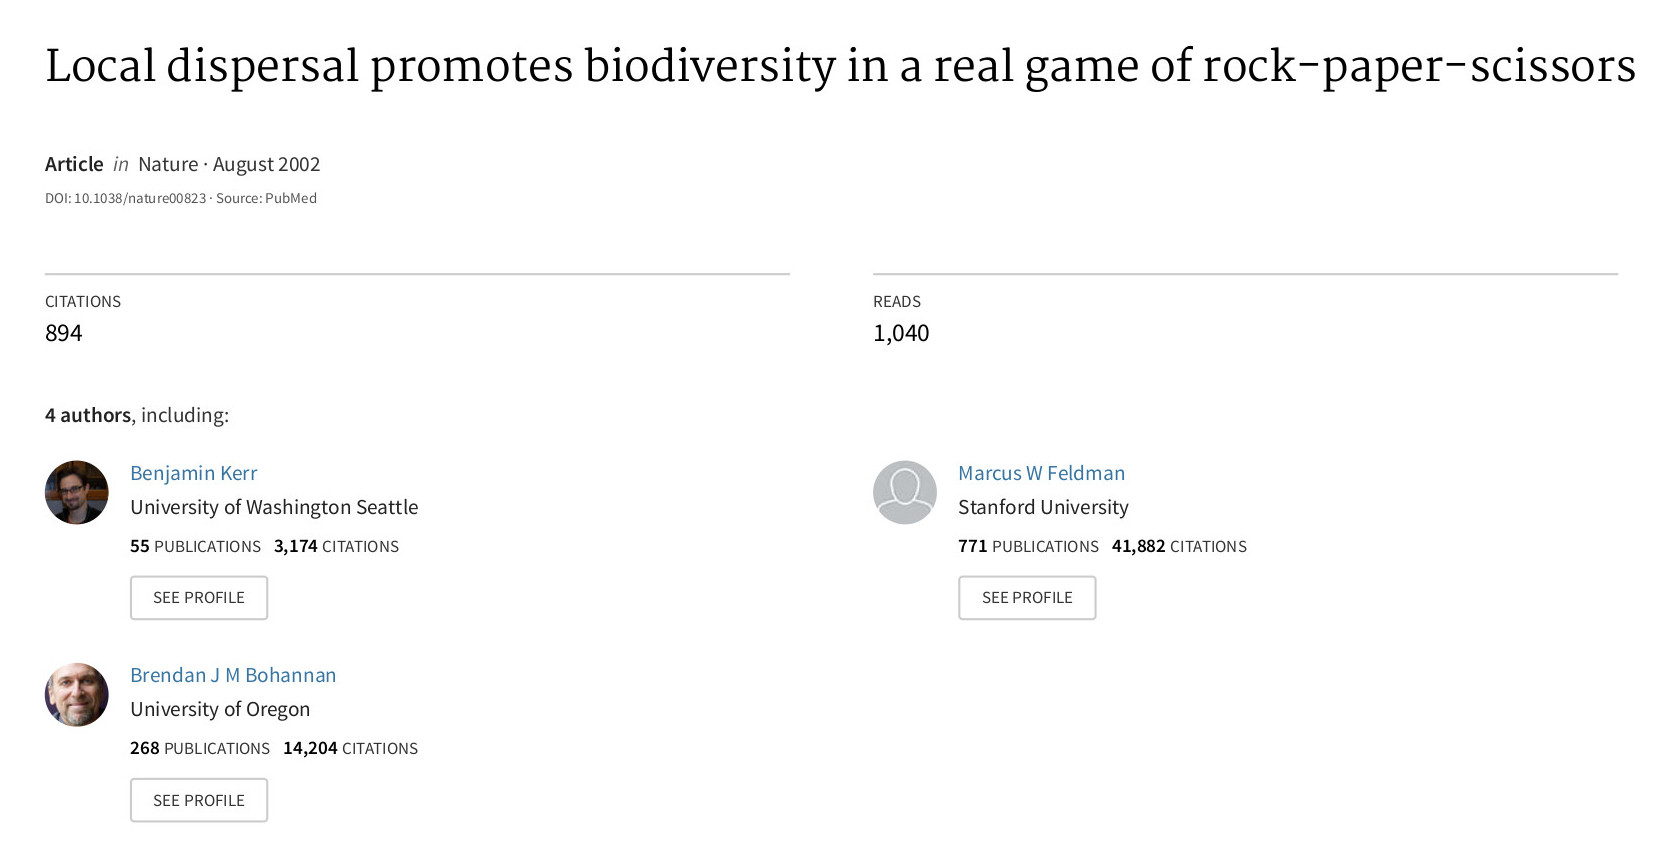
\includegraphics[scale=0.7]{img/paper_bacteria.jpg}
    		\end{figure}
\end{frame}

\begin{frame}{Rock-paper-scissors game in bacterial community}
    \begin{itemize}
		\item Three types of populations of \textit{E. coli}: 
		\begin{itemize}
			\item Wild-type bacterias (WT): colicin-sensitive bacterias (killed by colicin). 
			\item Colicinogenic bacterias (C): produce colicin toxin and are resistant to it.
			\item Colicin-resistant bacterias (R): WT bacterias resistant to colicin.
		\end{itemize}
		\item Parameters that describe the relationships of WT-C-R community:
		\begin{itemize}
			\item $a$: advantage of WT over R $\Rightarrow$ R consume a lot of energy, WT have not this problem.
			\item $b$: advantage of C over WT $\Rightarrow$ C are able to kill WT.
			\item $c$: advantage of R over C $\Rightarrow$ R are resistant to colicin produced by C. 
		\end{itemize}
		
    \end{itemize}
\end{frame}

\begin{frame}{Rock-paper-scissors game in bacterial community}
	\begin{columns}
		\begin{column}{0.5\textwidth}
			\begin{center}
				In summary, we have the relationships of rock-paper-scissors game:
			\end{center}
			\begin{figure}
				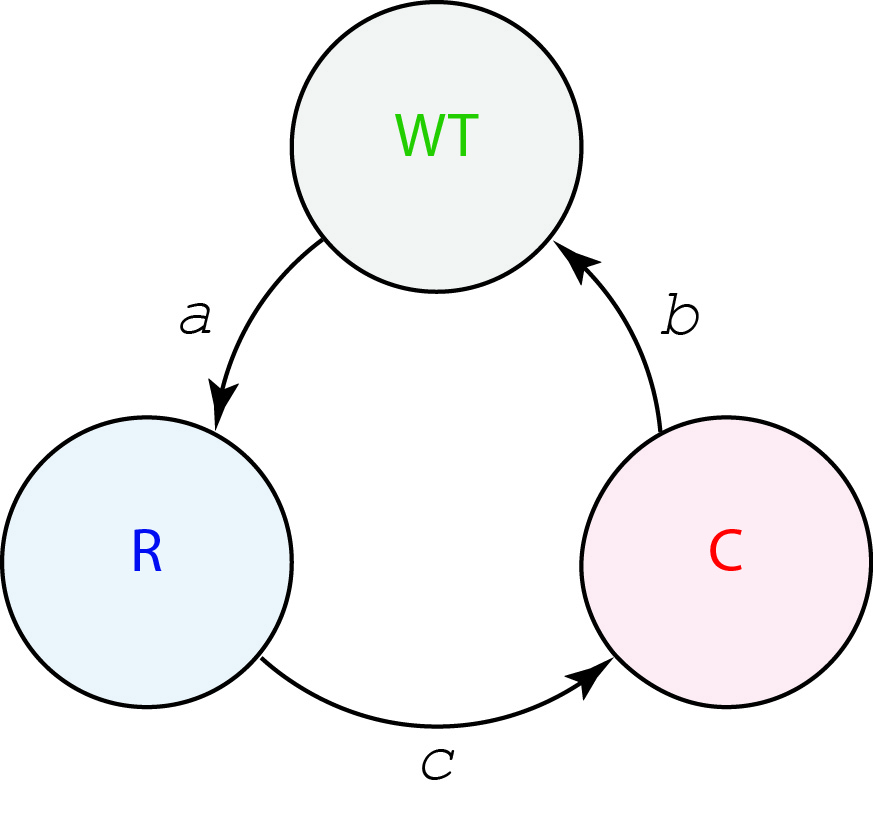
\includegraphics[scale=0.12]{img/figure_rock-scissor-paper.jpg}			
			\end{figure}
		\end{column}
		\begin{column}{0.5\textwidth}
			\begin{center}
				And the resulting equations:
			\begin{align*}
				W\left(WT\right) = 1 + af_R - bf_C\\
				W\left(C\right) = 1 + bf_{WT} - cf_R\\
				W\left(R\right) = 1 + cf_C - af_{WT}\\
			\end{align*}
			where $f_{WT}$, $f_C$ and $f_R$ are the frequencies of WT, C and R, respectively. 
			\end{center}
		\end{column}
	\end{columns}
	\pause
	\begin{center}
		{\LARGE $\Downarrow$\\}
		%% Meter alert %%
		\begin{block}
			{\centering
<<<<<<< HEAD
				Simulations 
=======
				Simulations
>>>>>>> 69670d7ba615fee5d0c09611326fc2936108c963
			}
		\end{block}
	\end{center}	
\end{frame}


\begin{frame}{Rock-paper-scissors game in bacterial community}
Case 1: a = b = c = 1
	\begin{columns}
		\begin{column}{0.5\textwidth}
			\begin{figure}
				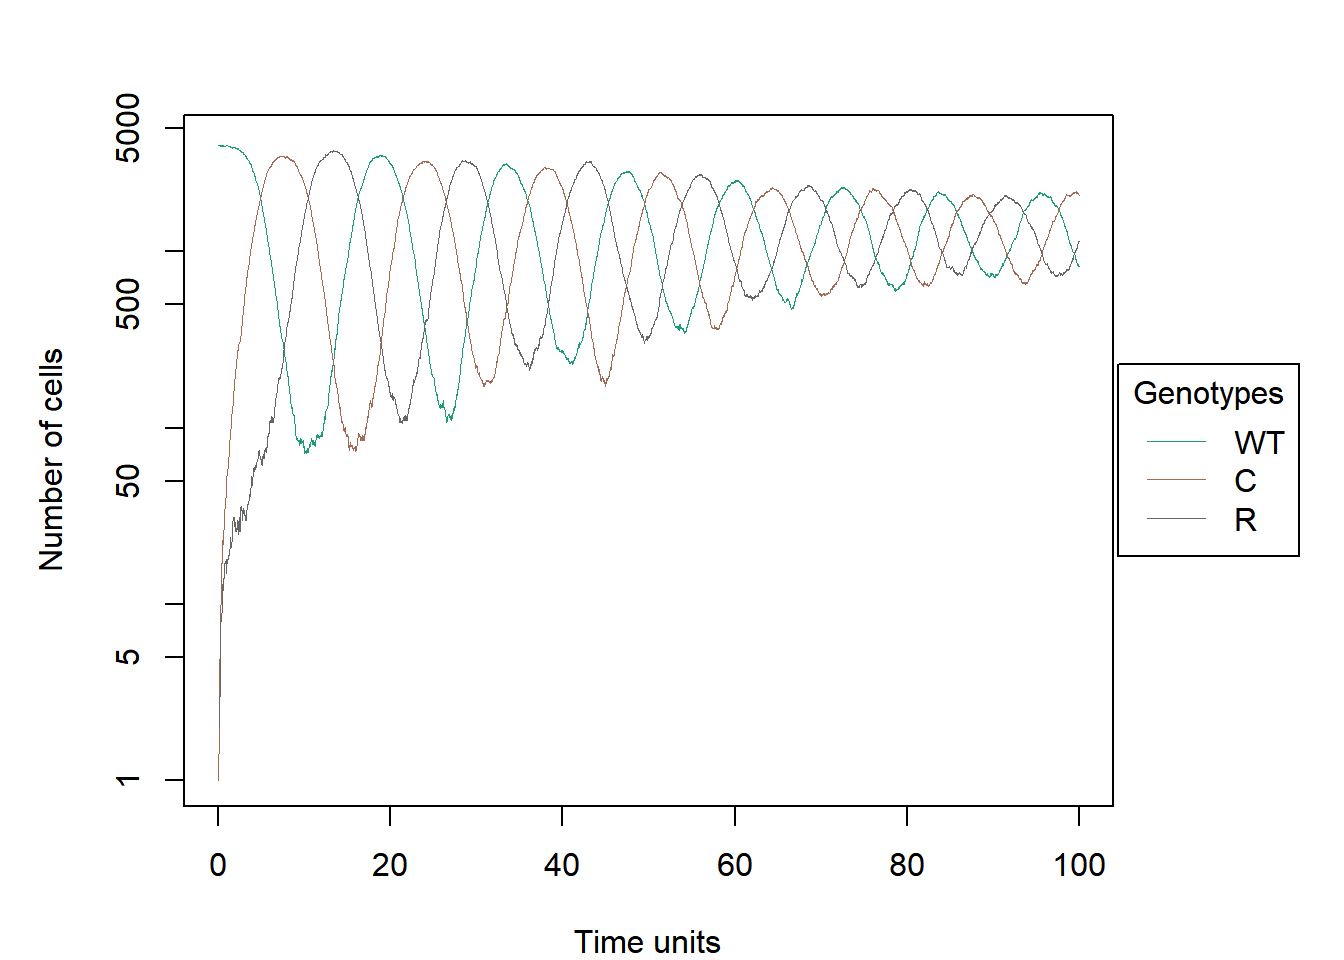
\includegraphics[scale=0.35]{img/CRS_caso1_1.png}			
			\end{figure}
		\end{column}

		\begin{column}{0.5\textwidth}
			\begin{figure}
				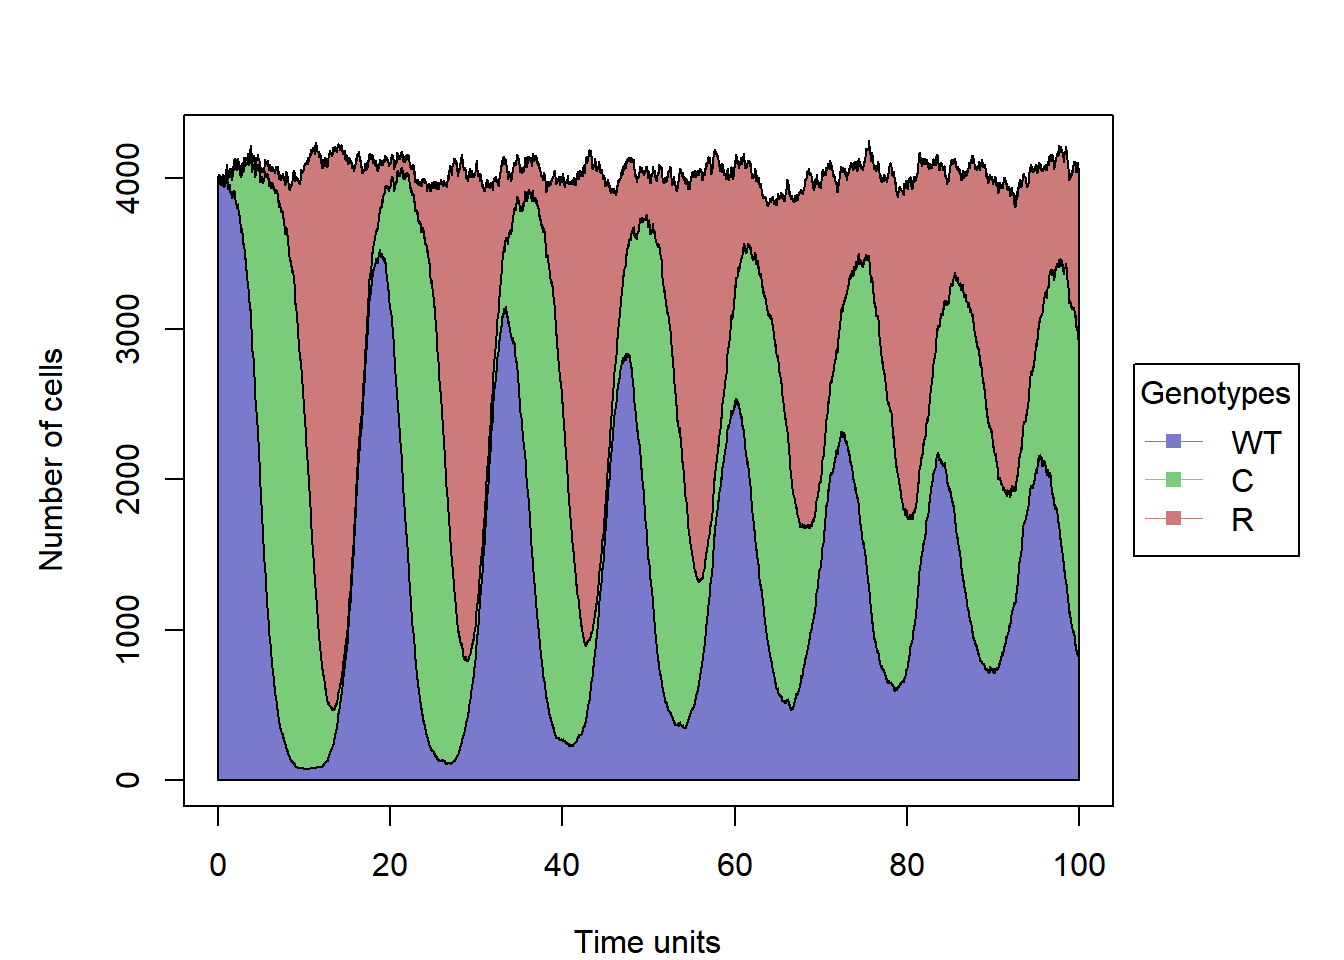
\includegraphics[scale=0.35]{img/CRS_caso1_2.png}			
			\end{figure}
		\end{column}
	\end{columns}
\end{frame}

\begin{frame}{Rock-paper-scissors game in bacterial community}
Case 2: a = 10,  b = c = 1
	\begin{columns}
		\begin{column}{0.5\textwidth}
			\begin{figure}
				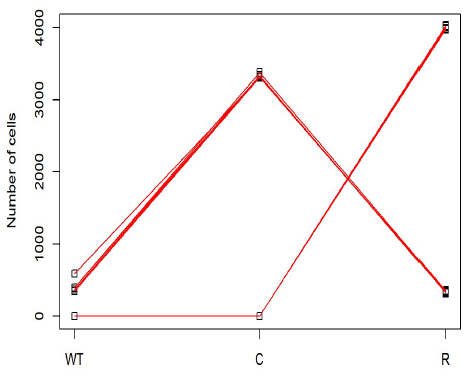
\includegraphics[scale=0.35]{img/CRS_caso2_1.png}			
			\end{figure}
		\end{column}

		\begin{column}{0.5\textwidth}
			\begin{figure}
				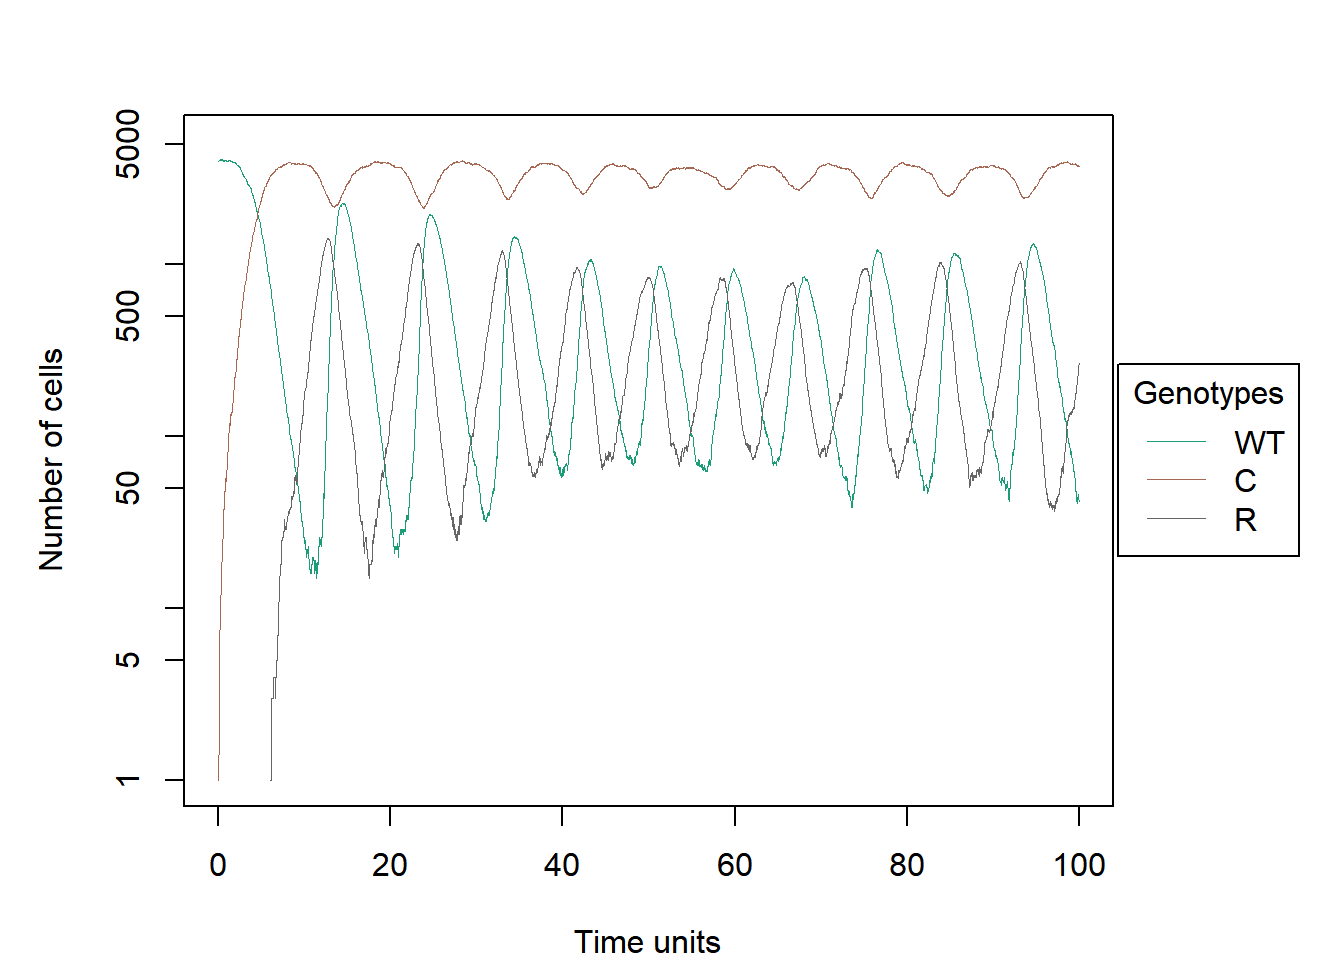
\includegraphics[scale=0.35]{img/CRS_caso2_2.png}			
			\end{figure}
		\end{column}
	\end{columns}
\end{frame}

\begin{frame}{Rock-paper-scissors game in bacterial community}
Case 2: a = 10,  b = c = 1
	\begin{columns}
		\begin{column}{0.5\textwidth}
			\begin{figure}
				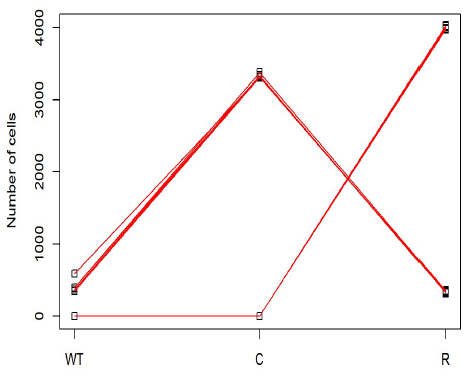
\includegraphics[scale=0.35]{img/CRS_caso2_1.png}			
			\end{figure}
		\end{column}

		\begin{column}{0.5\textwidth}
			\begin{figure}
				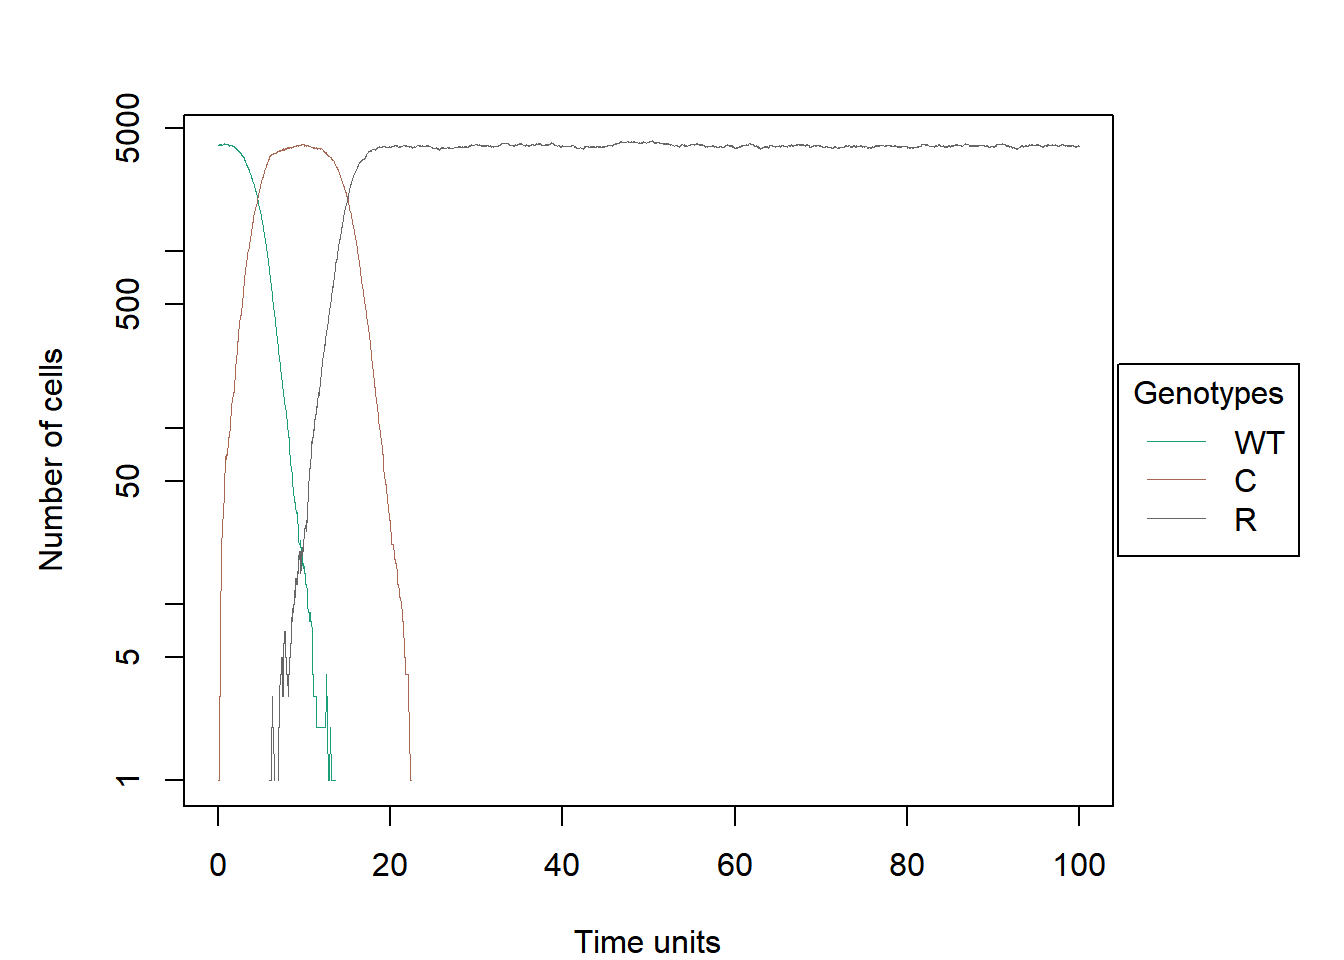
\includegraphics[scale=0.35]{img/CRS_caso2_3.png}			
			\end{figure}
		\end{column}
	\end{columns}
\end{frame}

\subsection{An experiment with cells}

\begin{frame}{Tumour-Stroma Interactions}

    \begin{itemize}
        \item \textbf{Title:} Evolutionary Dynamics of Tumor-Stroma Interactions in Multiple Myeloma.
        \item \textbf{Authors:} Javad Salimi Sartakhti, Mohammad Hossein Manshaei, Soroosh Bateni, Marco Archetti.
        \item Cancer cells and stromal cells cooperate by exchanging diffusible factors.
        \begin{itemize}
            \item Frequency-dependent selection that can be studied in the framework of evolutionary game theory.
        \end{itemize}
    \end{itemize}
    
\end{frame}

\begin{frame}{Tumour-Stroma Interactions: payoff functions}
    \begin{itemize}
        \item There are $n$ phenotypes in a population denoted by $\{ P_1, \ldots, P_n \}$.
        \item Each phenotype can produce one diffusible factor $\{ G_1, \ldots, G_n \}$.
        \item Each diffusible factor $j$ has a different effect $r_{i,j}$ on the other phenotypes $i$.
        \item The cost for $P_i$ for growth factor $G_i$ is denoted as $c_i$.
        \item $M$ is the number of cells within the diffusion range.
        \begin{itemize}
            \item There are $M_j$ individuals of type $P_j$ among the other group members.
        \end{itemize}
        \item The payoff for strategy $P_j$ is:
        \begin{align*}
            \pi_{P_j}(M_1,\ldots,M_n)=\frac{(M_j+1)\times c_j}{M}r_{j,j} + \sum_{i=1, i \neq j}^n \frac{M_i \times c_i}{M}r_{j,i} - c_j \;.
        \end{align*}
    \end{itemize}
\end{frame}

\begin{frame}{Tumour-Stroma Interactions: dynamics}
    \begin{columns}
        \begin{column}{0.4\textwidth}
             \begin{itemize}
                \item Malignant plasma cells.
                \item Osteoblasts.
                \item Osteoclasts.
                \item Growth factors:
                \begin{itemize}
                    \item Autocrine effects.
                    \item Paracrine effects. 
                \end{itemize}
            \end{itemize}
        \end{column}
        \begin{column}{0.6 \textwidth}
            \begin{figure}[t]
                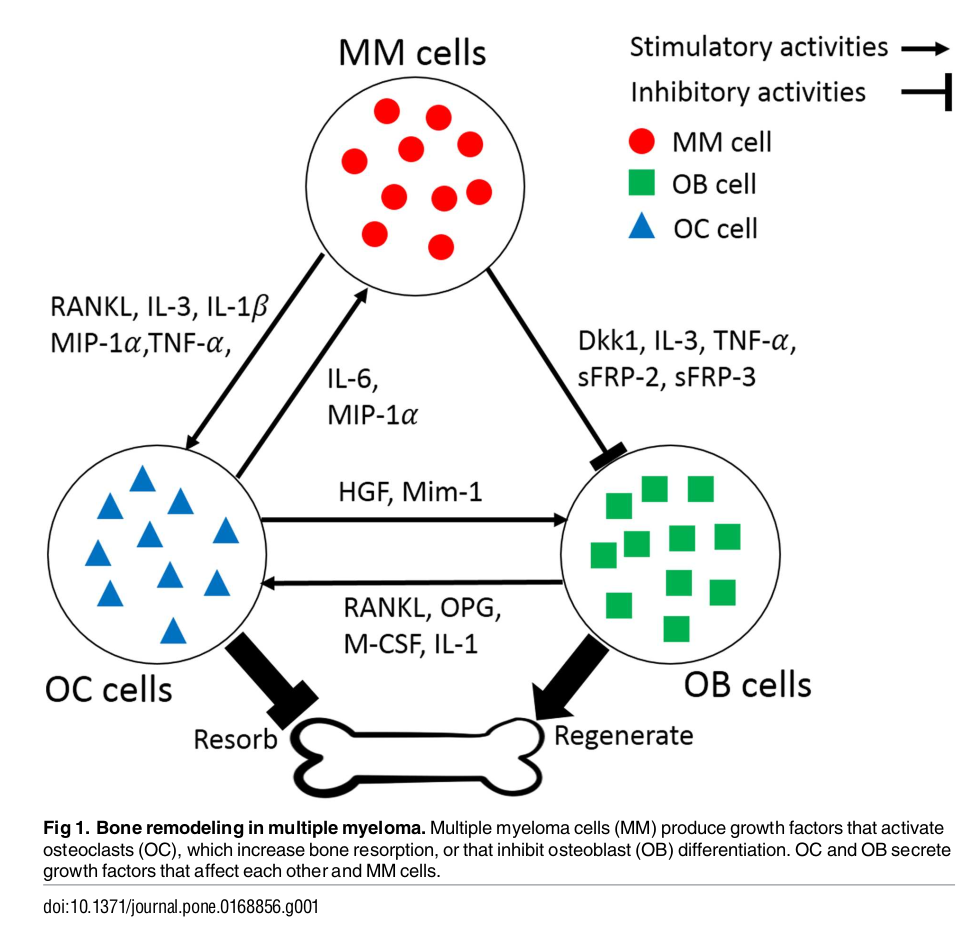
\includegraphics[width=0.9\linewidth]{img/tumour_stroma_interactions.png}
            \end{figure}
        \end{column}
    \end{columns}
\end{frame}



\begin{frame}{Tumour-Stroma Interactions: Scenario 1}
    \begin{itemize}
        \item $c_1<c_2<c_3$ (a common occurrence in multiple myeloma).
        \item In the presence of a small number of MM cells, the stable point on the OB-OC border becomes a saddle point and clonal selection leads to a stable coexistence of OC and MM cells.
    \end{itemize}
    
    \begin{columns}
        \begin{column}{0.4\textwidth}
            \begin{figure}[t]
                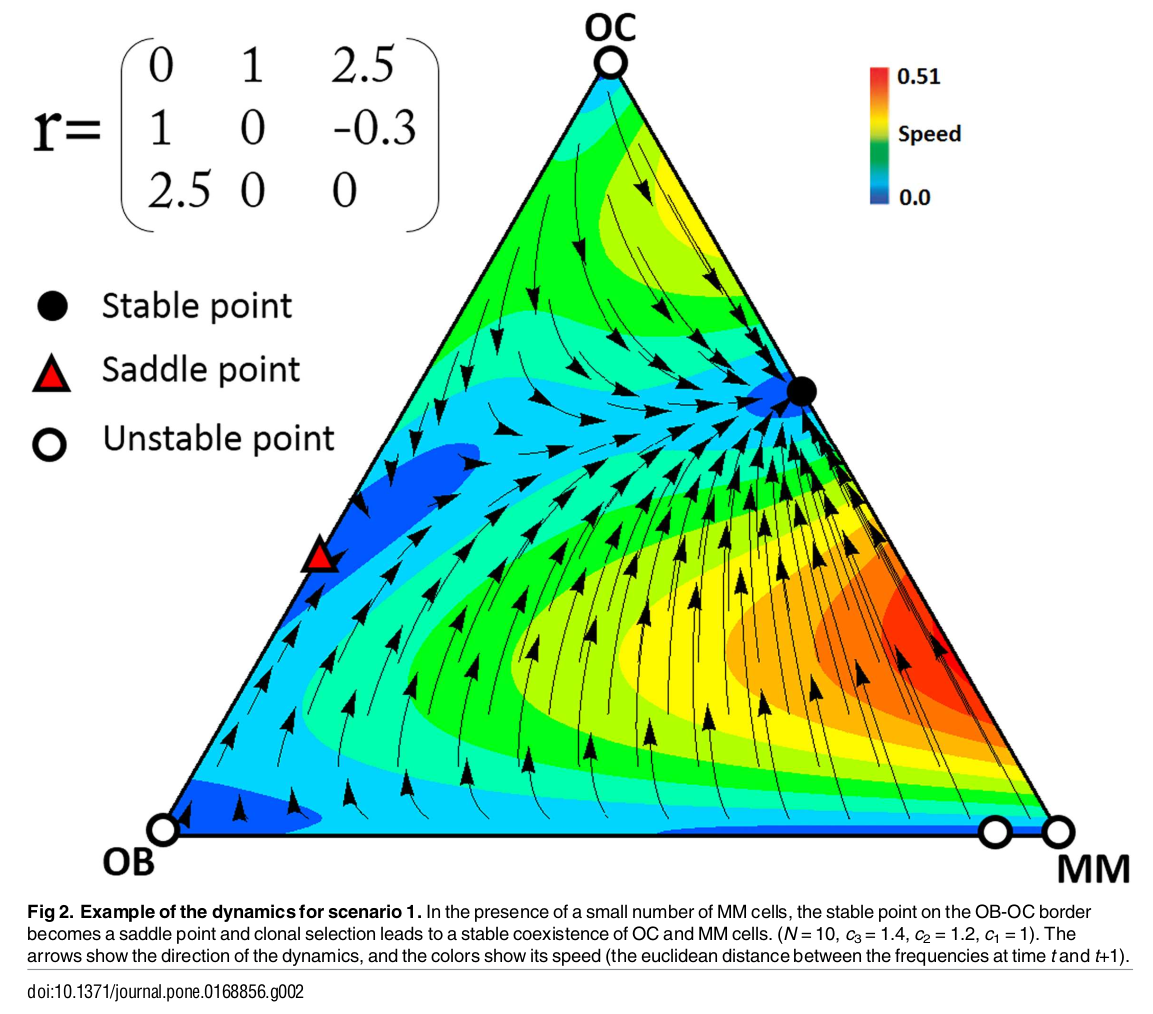
\includegraphics[width=0.9\linewidth]{img/Scenario1.png}
            \end{figure}
        \end{column}
        \begin{column}{0.6\textwidth}
            \begin{figure}[t]
                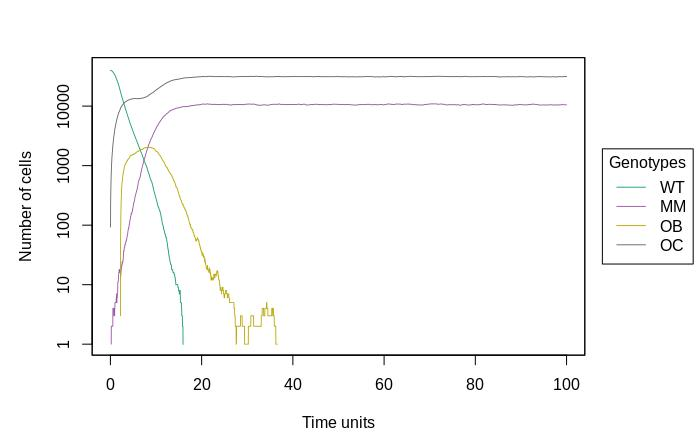
\includegraphics[width=0.9\linewidth]{img/scenario1_tr.jpg}
            \end{figure}
        \end{column}
    \end{columns}
\end{frame}

\begin{frame}{Tumour-Stroma Interactions: Scenario 2}
    \begin{itemize}
        \item $c_1=c_2=c_3$.
        \item The game has one polymorphic stable point between OB and OC. In this case, clonal selection leads to the regular OC-OB balance and prevents invasion of MM cells.
    \end{itemize}
    
    \begin{columns}
        \begin{column}{0.4\textwidth}
            \begin{figure}[t]
                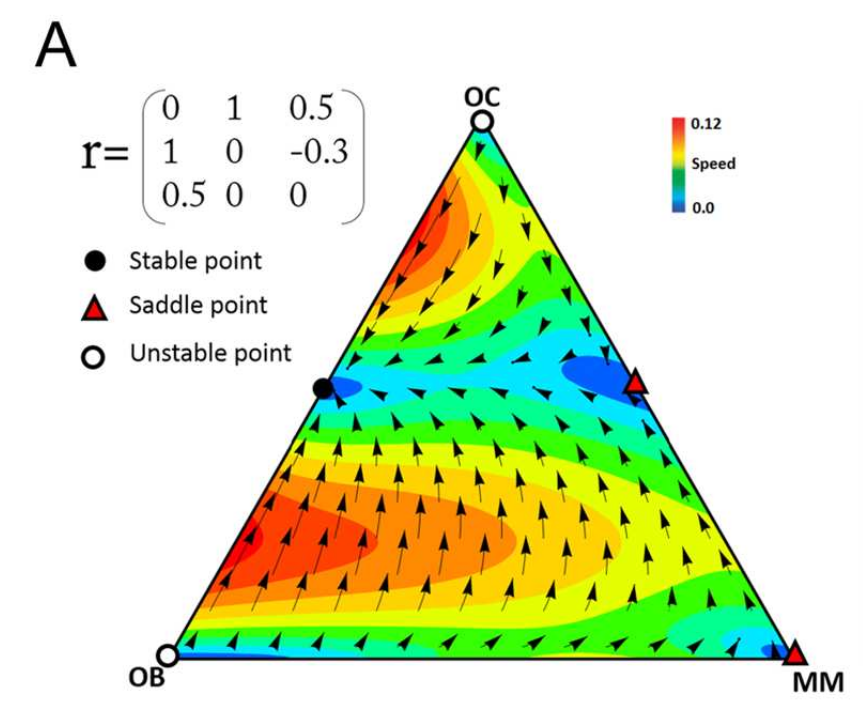
\includegraphics[width=0.9\linewidth]{img/Scenario2.png}
            \end{figure}
        \end{column}
        \begin{column}{0.6\textwidth}
            \begin{figure}[t]
                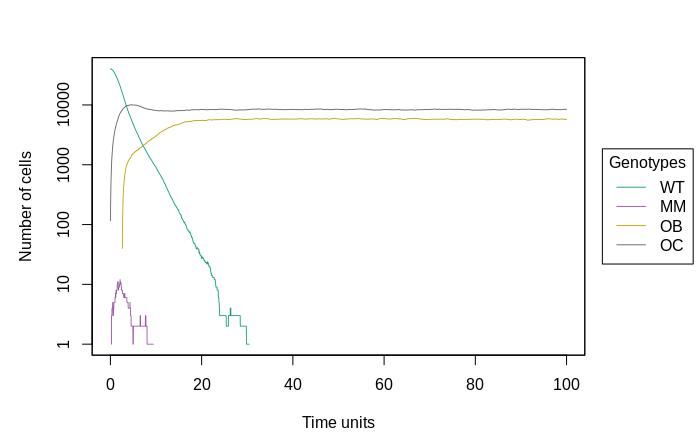
\includegraphics[width=0.9\linewidth]{img/scenario2_tr.jpg}
            \end{figure}
        \end{column}
    \end{columns}
\end{frame}

\section{ProbCons}
\begin{frame}{Algorithm overview}
    \begin{itemize}
        \item \textbf{ProbCons\cite{do2005probcons}} is a pair-hidden Markov model-based progressive alignment algorithm that differs from most typical approaches in its use of \textbf{maximum expected accuracy} rather than Viterbi alignment, and of the probabilistic consistency transformation to incorporate multiple sequence conservation information during pairwise alignment. 
        \item \textbf{Hidden Markov Models (HMMs)} in sequence analysis are based on a strong probabilistic model that \textbf{includes a representation of INDELs} (insertions and deletions, i.e. gaps). 
        \item The HMM describing families of related sequences are called \textbf{profile HMMs}
    \end{itemize}
\end{frame}

\begin{frame}{Algorithm overview}
    \begin{itemize}
        \item In profile HMMs the residues in each position of the alignment can be in one of three possible states:
        \begin{enumerate}
            \item \textbf{Match:} represent conserved position
            \item \textbf{Insert:} represent small stretches of nonspecific sequence
            \item \textbf{Delete:} correspond to gaps and represent the absence of a conserved residue
        \end{enumerate}
        \item Each state has associated:
        \begin{enumerate}
            \item \textbf{Emission probability:} correspond to the probability of observing each amino acid at that particular position of the alignment
            \item \textbf{Transition probability:} describes the frequency of observing a match, insertion or deletion in column i+1 given the state column i. 
        \end{enumerate}
    \end{itemize}
    
\end{frame}

\begin{frame}{Algorithm overview}
\centering
 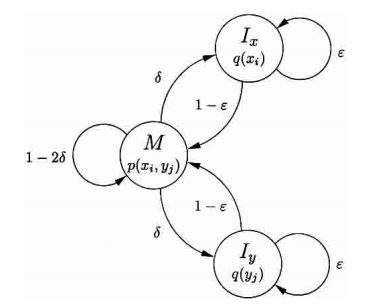
\includegraphics[width=0.35\linewidth]{img/hmm_states.PNG}
 \begin{itemize}
     \item Emission probabilities, which correspond to traditional substitution scores, are based on the BLOSUM62 matrix.
     \item Transition probabilities, which correspond to gap penalties, are trained with unsupervised Expectation-Maximization (EM)
     \begin{itemize}
         \item $\pi_{insert}$: initial insertion probability parameter
         \item $\delta$: insertion start probability parameter
         \item $\epsilon$: insertion extension probability parameter
     \end{itemize}
     \item The resulting parameters ($\delta$ = 0.019931, $\epsilon$ = 0.79433, $\pi_{insert}$= 0.19598) are used as the default for the program.

 \end{itemize}
    
\end{frame}

\begin{frame}
    \frametitle{Algorithm overview}

    \begin{block}{ProbCons \cite{do2005probcons}}
        \begin{itemize}
            \item Given $m$ sequences $\rightarrow$ $S = \{s^{(1)}, \ldots, s^{(m)} \}$.
            \item Maximum expected accuracy.
            \item Probabilistic consistency $\rightarrow$ MSA conservation information in the pairwise alignment.
        \end{itemize}
    \end{block}
    
    \begin{enumerate}
        \item Step 1: Computation of posterior probability matrices.
        \item Step 2: Computation of expected accuracies.
        \item Step 3: Probabilistic consistency transformation.
        \item Step 4: Computation of the guide tree.
        \item Step 5: Progressive alignment.
        \item Step 6: Iterative refinement (post-processing OPTIONAL step).
    \end{enumerate}
\end{frame}

\begin{frame}
    \frametitle{Step 1: Computation of posterior probability matrices}
    \begin{itemize}
        \item For $x, y \in S$, compute the matrix
        \begin{align*}
            P_{xy}(i,j) = \pmb{P}(x_i \sim y_j \in a^* | x, y) \;,
        \end{align*}
        where $1\leq i\leq|x|$ and $1\leq j\leq |y|$.
        \item Each position $P_{xy}(i,j)$ is the \textbf{posterior} probability that letters $x_i$ and $y_j$ are paired i an alignment $a^*$.
        \begin{itemize}
            \item Computing posterior probabilities in pair-HMMs \cite{durbin1998biological}.
        \end{itemize}
        \item Time complexity $O(m^2 L^2)$.
        \begin{itemize}
            \item $m$ is the number of sequences.
            \item $L$ is the length of each sequence.
        \end{itemize}
    \end{itemize}
\end{frame}

\begin{frame}
    \frametitle{Step 2: Computation of expected accuracies}
    \begin{itemize}
        \item The expected accuracy is defined as
        \begin{align*}
            \pmb{E}_{a^*} (acc(a,a^*)|x,y) = \frac{1}{\min{\{|x|,|y|\}}} \sum_{x_i\sim y_j \in a} P_{xy}(i,j) \;,
        \end{align*}
        where $a$ is the align*ment that maximizes the expected accuracy by dynamic programming.
        \item Set 
        \begin{align}\label{eq:score}
            E(x,y) = \pmb{E}_{a^*} (acc(a,a^*)|x,y) \;.
        \end{align}
    \end{itemize}
\end{frame}

\begin{frame}
    \frametitle{Step 3: Probabilistic consistency transformation}
    \begin{itemize}
        \item Reestimate quality scores $\pmb{P}_{xy}$ $\rightarrow$ probabilistic consistency transformation.
        \item Incorporate similarity of $x$ and $y$ to other sequences in $S$:
        \begin{align*}
            {\pmb{P}}'(x_i \sim y_j \in a^* | x, y) = \frac{1}{|S|} \sum_{z\in S} \sum_{z_k \in z} F(x_i, y_j, z_k) \;,
        \end{align*}
        where $F(x_i, y_j, z_k) =  {\pmb{P}}(x_i \sim z_k \in a^* | x, z) \times {\pmb{P}}(z_k \sim y_j \in a^* | z, y) $.
        \item In matrix form:
        \begin{align*}
            {P'}_{xy} = \frac{1}{|S|} \sum_{z\in S} P_{xz}P_{zy} \;.
        \end{align*}
        \item \textbf{Optimization: }use sparse matrices ignoring entries $\leq \omega$ (threshold).
        \item This step can be iterated until convergence.
    \end{itemize}
\end{frame}

\begin{frame}
    \frametitle{Steps 4, 5 and 6}
    \begin{itemize}
        \item Hierarchical clustering.
        \begin{itemize}
          \item Similarity measure $E(x,y)$ as defined in Equation \eqref{eq:score}.
          \item WPGMA method.
        \end{itemize}
        \item Align sequence groups hierarquically.
        \begin{itemize}
            \item Sum-of-pairs.
            \item Gap penalties $\rightarrow$ $0$.
        \end{itemize}
        \item Progressive alignment.
        \begin{itemize}
            \item Randomly partition alignment into two groups of sequences.
            \item Realign.
            \item This step can be iterated.
        \end{itemize}
    \end{itemize}
    
\end{frame}

\section{Examples}
\begin{frame}{Examples: Comparison between methods}

    \begin{itemize}
        \item MSA of distantly related globins (human beta globin, human myoglobin, human neuroglobin, soybean leghemoglobin, rice hemoglobin) using four different programs. Symbols: * complete conservation, : conservative substitutions, . less conservative substitutions. Programs differ in:
        \begin{itemize}
            \item Align corresponding regions of alpha helical secondary structure (red lettering).
            \item Align conserved histidines (open and black arrowhead). They are important in coordinating protein binding to the heme group $\rightarrow$ they should be aligned by all the programs. The open arrowhead histidine shows a complete conservation. The conservation of the black is only achieved by ProbCons and T-Coffee.
            \item Create and place gaps (boxed regions).
        \end{itemize}
    \end{itemize}
            
\end{frame}

\begin{frame}

    \begin{figure}[t]
        \raggedleft
        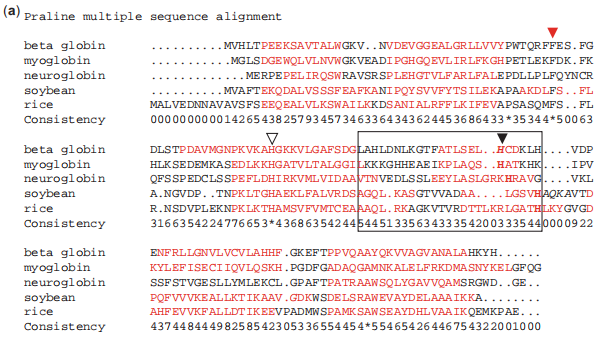
\includegraphics[width=0.49\textwidth]{./img/Comparacion_1.png}
        \raggedright
        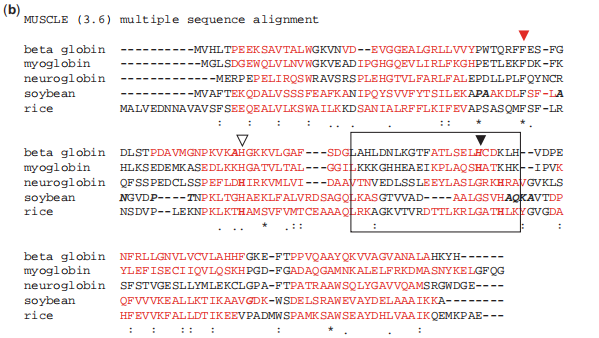
\includegraphics[width=0.49\textwidth]{./img/Comparacion_2.png}
    \end{figure}
    \begin{figure}[b]
        \raggedleft
        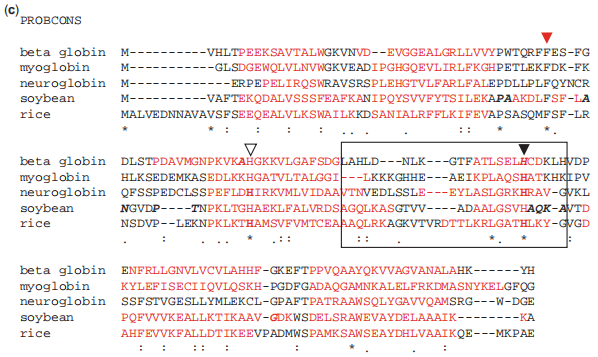
\includegraphics[width=0.49\textwidth]{./img/Comparacion_3.png}
        \raggedright
        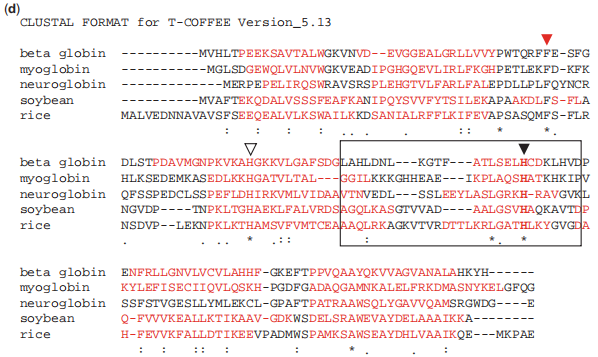
\includegraphics[width=0.49\textwidth]{./img/Comparacion_4.png}
    \end{figure}

\end{frame}

%%%%%%%% greetings %%%%%%%%
\frame{\titlepage}
%------------------------------------------------



\end{document}